% Options for packages loaded elsewhere
\PassOptionsToPackage{unicode}{hyperref}
\PassOptionsToPackage{hyphens}{url}
%
\documentclass[
  ignorenonframetext,
  aspectratio=169]{beamer}
\usepackage{pgfpages}
\setbeamertemplate{caption}[numbered]
\setbeamertemplate{caption label separator}{: }
\setbeamercolor{caption name}{fg=normal text.fg}
\beamertemplatenavigationsymbolsempty
% Prevent slide breaks in the middle of a paragraph
\widowpenalties 1 10000
\raggedbottom
\setbeamertemplate{part page}{
  \centering
  \begin{beamercolorbox}[sep=16pt,center]{part title}
    \usebeamerfont{part title}\insertpart\par
  \end{beamercolorbox}
}
\setbeamertemplate{section page}{
  \centering
  \begin{beamercolorbox}[sep=12pt,center]{section title}
    \usebeamerfont{section title}\insertsection\par
  \end{beamercolorbox}
}
\setbeamertemplate{subsection page}{
  \centering
  \begin{beamercolorbox}[sep=8pt,center]{subsection title}
    \usebeamerfont{subsection title}\insertsubsection\par
  \end{beamercolorbox}
}
\AtBeginPart{
  \frame{\partpage}
}
\AtBeginSection{
  \ifbibliography
  \else
    \frame{\sectionpage}
  \fi
}
\AtBeginSubsection{
  \frame{\subsectionpage}
}
\usepackage{amsmath,amssymb}
\usepackage{iftex}
\ifPDFTeX
  \usepackage[T1]{fontenc}
  \usepackage[utf8]{inputenc}
  \usepackage{textcomp} % provide euro and other symbols
\else % if luatex or xetex
  \usepackage{unicode-math} % this also loads fontspec
  \defaultfontfeatures{Scale=MatchLowercase}
  \defaultfontfeatures[\rmfamily]{Ligatures=TeX,Scale=1}
\fi
\usepackage{lmodern}
\usetheme[]{Frankfurt}
\usecolortheme{orchid}
\ifPDFTeX\else
  % xetex/luatex font selection
\fi
% Use upquote if available, for straight quotes in verbatim environments
\IfFileExists{upquote.sty}{\usepackage{upquote}}{}
\IfFileExists{microtype.sty}{% use microtype if available
  \usepackage[]{microtype}
  \UseMicrotypeSet[protrusion]{basicmath} % disable protrusion for tt fonts
}{}
\makeatletter
\@ifundefined{KOMAClassName}{% if non-KOMA class
  \IfFileExists{parskip.sty}{%
    \usepackage{parskip}
  }{% else
    \setlength{\parindent}{0pt}
    \setlength{\parskip}{6pt plus 2pt minus 1pt}}
}{% if KOMA class
  \KOMAoptions{parskip=half}}
\makeatother
\usepackage{xcolor}
\newif\ifbibliography
\setlength{\emergencystretch}{3em} % prevent overfull lines
\providecommand{\tightlist}{%
  \setlength{\itemsep}{0pt}\setlength{\parskip}{0pt}}
\setcounter{secnumdepth}{-\maxdimen} % remove section numbering
\setbeamertemplate{itemize items}[default]
\setbeamertemplate{enumerate items}[default]
\setbeamertemplate{navigation symbols}{}
\setbeamercolor{section in head/foot}{fg=white}
\setbeamercolor{itemize item}{fg=black}
\setbeamercolor{structure}{fg=black}

\usepackage{tabularx, graphicx, longtable, multicol, booktabs,
  listings, graphicx, amsmath, amsfonts, amssymb, tikz, pdfpages,
  multirow, collcell, epigraph, adjustbox, siunitx, colortbl}
\usepackage{mathrsfs}
\usepackage[T1]{fontenc}
\usepackage{lmodern}
\usepackage{appendixnumberbeamer}
\usetikzlibrary{shapes.geometric, arrows.meta, positioning}
\tikzstyle{circle_style} = [circle, draw, thick, minimum size=3cm, text centered, font=\large]
\tikzstyle{arrow_style} = [ultra thick, ->, >=latex, rounded corners=12pt]

\setbeamertemplate{footline}
{\begin{beamercolorbox}[sep=1ex]{author in head/foot}
  \hfill\llap{\insertframenumber}%
  \end{beamercolorbox}%
}

\AtBeginPart{}
\AtBeginSubsection{}
\AtBeginSubsubsection{}
\setlength{\emergencystretch}{0em}
\setlength{\parskip}{0pt}

\AtBeginSection{}


% Shaded Quote

\usepackage{etoolbox, framed, libertine}
\newcommand*\quotefont{\fontfamily{LinuxLibertineT-LF}}

\newcommand*\quotesize{60} % if quote size changes, need a way to make shifts relative
% Make commands for the quotes
\newcommand*{\openquote}
   {\tikz[remember picture,overlay,xshift=-4ex,yshift=-2.5ex]
   \node (OQ) {\quotefont\fontsize{\quotesize}{\quotesize}\selectfont``};\kern0pt}

\newcommand*{\closequote}[1]
  {\tikz[remember picture,overlay,xshift=4ex,yshift={#1}]
   \node (CQ) {\quotefont\fontsize{\quotesize}{\quotesize}\selectfont''};}

% select a colour for the shading
\colorlet{shadecolor}{white}

\newcommand*\shadedauthorformat{\emph} % define format for the author argument

% Now a command to allow left, right and centre alignment of the author
\newcommand*\authoralign[1]{%
  \if#1l
    \def\authorfill{}\def\quotefill{\hfill}
  \else
    \if#1r
      \def\authorfill{\hfill}\def\quotefill{}
    \else
      \if#1c
        \gdef\authorfill{\hfill}\def\quotefill{\hfill}
      \else\typeout{Invalid option}
      \fi
    \fi
  \fi}
% wrap everything in its own environment which takes one argument (author) and one optional argument
% specifying the alignment [l, r or c]
%
\newenvironment{shadequote}[2][l]%
{\authoralign{#1}
\ifblank{#2}
   {\def\shadequoteauthor{}\def\yshift{-2ex}\def\quotefill{\hfill}}
   {\def\shadequoteauthor{\par\authorfill\shadedauthorformat{#2}}\def\yshift{2ex}}
\begin{snugshade}\begin{quote}\openquote}
{\shadequoteauthor\quotefill\closequote{\yshift}\end{quote}\end{snugshade}}
\usepackage{booktabs}
\usepackage{longtable}
\usepackage{array}
\usepackage{multirow}
\usepackage{wrapfig}
\usepackage{float}
\usepackage{colortbl}
\usepackage{pdflscape}
\usepackage{tabu}
\usepackage{threeparttable}
\usepackage{threeparttablex}
\usepackage[normalem]{ulem}
\usepackage{makecell}
\usepackage{xcolor}
\usepackage{bookmark}
\IfFileExists{xurl.sty}{\usepackage{xurl}}{} % add URL line breaks if available
\urlstyle{same}
\hypersetup{
  hidelinks,
  pdfcreator={LaTeX via pandoc}}

\author{}
\date{\vspace{-2.5em}}

\begin{document}

\begin{frame}
\title{Attraction Effect in Risky Choices}
\author{Yi-tsen Liao}
\institute{Carnegie Mellon University Social Decision Science}
\date{Sep 29, 2025\\BDR Lab Meeting}

\maketitle
\end{frame}

\section{Introduction}\label{introduction}

\subsection{Intro}\label{intro}

\begin{frame}{Context Effect}
\phantomsection\label{context-effect}
\begin{itemize}
  \item When choosing among options with multiple attributes
  \pause
  \item We often face difficult situations where one option is better in some domains,
  \pause
  \item while the alternative is better in the other domains
\end{itemize}

\vfill

\begin{center}
\pause
  \textbf{Choosing partner, houses hunting, buying cars...}
\end{center}
\end{frame}

\begin{frame}{Context Effect}
\phantomsection\label{context-effect-1}
\begin{center}
  \textbf{These choices may be influenced by other available options}
\end{center}

\pause
\begin{itemize}
  \item An option may be viewed differently when it is evaluated in isolation v.s. when it is jointly evaluated with other options (Hsee et al, 1999)
  \pause
  \item When making choices among options with multiple "aspects", we often compare them attribute by attribute (Tversky, 1972)
  \pause
  \item A choice between two options is affected by the
introduction of a third option (Trueblood et al, 2014)
\end{itemize}
\end{frame}

\begin{frame}{Context Effect}
\phantomsection\label{context-effect-2}
\begin{center}
  \textbf{Types of context effects vary by how the third option is constructed}
\end{center}

\pause
\begin{itemize}
  \item Attraction effect (Huber et al, 1982)
  \begin{itemize}
    \item The third option ("Decoy") is similar but inferior to the focal option 
    \item which enhances the probability of choosing the "similar but better" focal option
  \end{itemize}
  \pause
  \item Similarity effect (Tversky, 1972)
  \begin{itemize}
    \item The third option is similar to the non-focal option and DM is indifferent to all three options
    \item which enhances the probability of choosing the "unique" focal option
  \end{itemize}
  \pause
  \item Compromise effect (Simonson, 1989)
  \begin{itemize}
    \item The third is an extreme alternative to the focal option and DM is indifferent to all three options
    \item which enhances the probability of choosing the "moderate" focal option
  \end{itemize}
\end{itemize}

\vfill

\begin{center}
\pause
  \textbf{In this study, we focus on the attraction effect!}
\end{center}
\end{frame}

\begin{frame}{Attraction Effect}
\phantomsection\label{attraction-effect}
\begin{center}
  \textbf{Types of attraction effects also vary by how the "decoy" is constructed}
\end{center}

\pause
\begin{itemize}
  \item Frequency decoy
  \begin{itemize}
    \item The decoy is worse than the focal option in its \textbf{weak} attribute
  \end{itemize}
  \pause
  \item Range decoy
  \begin{itemize}
    \item The decoy is worse than the focal option in its \textbf{strong} attribute
  \end{itemize}
  \pause
  \item Range-Frequency decoy
  \begin{itemize}
    \item The decoy is worse than the focal option in \textbf{all} attributes
  \end{itemize}
\end{itemize}
\end{frame}

\begin{frame}{Literatures on Attraction Effect}
\phantomsection\label{literatures-on-attraction-effect}
\begin{itemize}
  \pause
  \item Less studies on the mechanism of how the attraction effect
  \pause
  \item Often compare between focal and non-focal option, instead of a control
  \pause
  \item Often assume these different types of decoys work in the same way
  \pause
  \item Different theories may predict different choices given the same choice set
\end{itemize}
\end{frame}

\begin{frame}{Application of Attraction Effect}
\phantomsection\label{application-of-attraction-effect}
\begin{center}
  \textbf{In pricing}
\end{center}
\begin{center}
  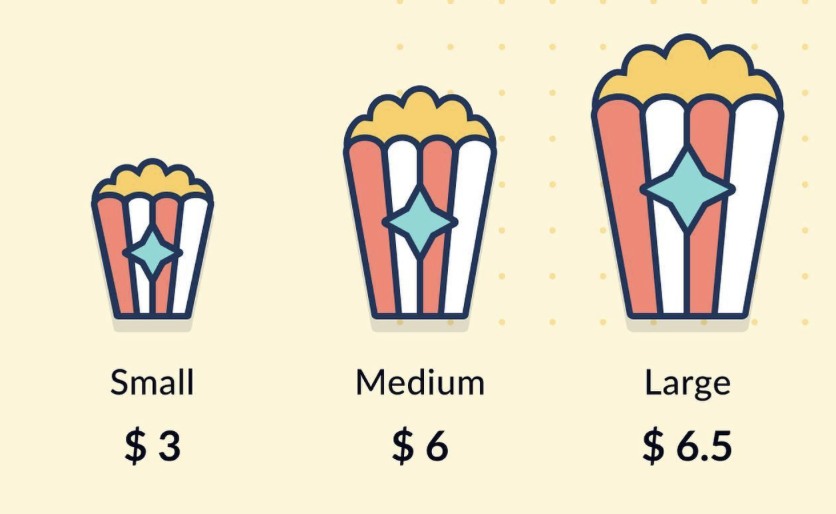
\includegraphics[width=0.6\textwidth]{intro_pricing.png}
\end{center}

\vfill

\hfill \tiny Source: @UXMental
\url{https://www.instagram.com/p/CsG2uBCNxO6/}
\end{frame}

\begin{frame}{Application of Attraction Effect}
\phantomsection\label{application-of-attraction-effect-1}
\begin{center}
  \textbf{In how we evaluate "beauty"}
\end{center}
\begin{center}
  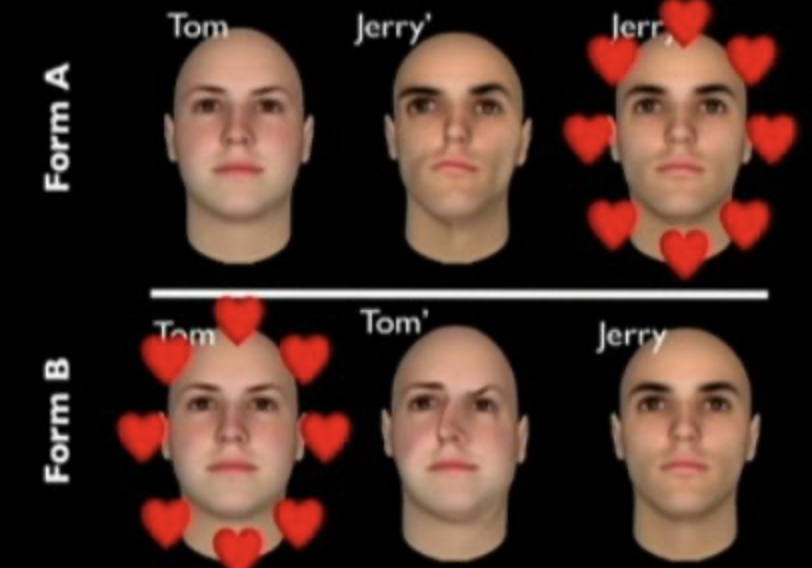
\includegraphics[width=0.6\textwidth]{intro_beauty.png}
\end{center}

\vfill

\hfill \tiny Source: @Dan Ariely
\url{https://www.youtube.com/watch?v=9X68dm92HVI}
\end{frame}

\begin{frame}{Application of Attraction Effect}
\phantomsection\label{application-of-attraction-effect-2}
\begin{center}
  \textbf{In visual perception...}
\end{center}
\begin{center}
  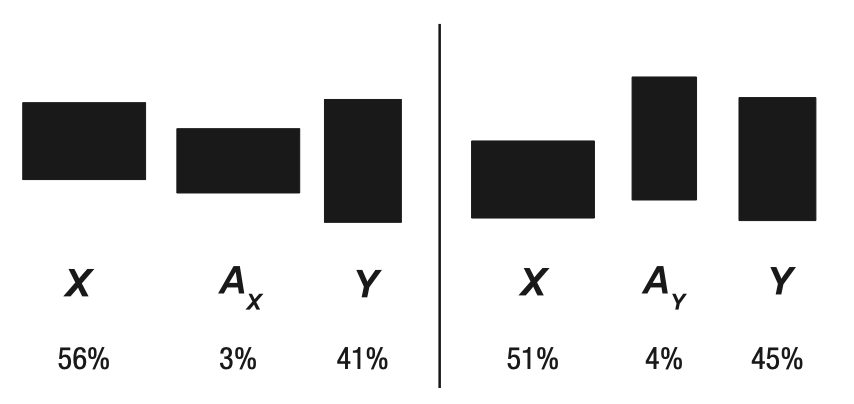
\includegraphics[width=0.6\textwidth]{intro_perception.png}
\end{center}

\vfill

\hfill \tiny Trueblood, J. S., Brown, S. D., Heathcote, A., \&
Busemeyer, J. R. (2013). Not just for consumers: Context effects are
fundamental to decision making. Psychological science, 24(6), 901-908.
\end{frame}

\begin{frame}{Limits of Studies on Attraction Effect}
\phantomsection\label{limits-of-studies-on-attraction-effect}
\begin{itemize}
  \pause
  \item Less studies on the mechanism of how attraction effect works exactly
  \pause
  \item Often compare between focal and non-focal option, instead of a control
  \pause
  \item Often assume these different types of decoys work in the same way
  \pause
  \item Different theories may predict different choices given the same choice set
\end{itemize}
\end{frame}

\begin{frame}{Limits of Studies on Attraction Effect}
\phantomsection\label{limits-of-studies-on-attraction-effect-1}
\begin{itemize}
  \item Has been widely studied in various fields, with real-world application
  \pause
  \item Caveat: they may not always work (Frederick et al, 2014)
  \pause
  \item Restricted to very limited number of options (most commonly 3)
  \pause
  \item with very limited number of attributes (most commonly 2)
\end{itemize}

\vfill
\begin{center}
  \textbf{What are the settings that are simplistic enough to fit into these narrow criteria?}
\end{center}

\begin{center}
  \pause
  \textbf{Good old lottery choices :)}
\end{center}
\end{frame}

\begin{frame}{Risky Choices}
\phantomsection\label{risky-choices}
\begin{itemize}
  \item People have a hard time thinking about risk
  \pause
  \item And we have a long history studying the inconsistency in choices under uncertainty
  \pause
  \item A lottery in some sense is an option with only two attributes: 
  \pause
  \begin{itemize}
    \item A set of prizes
    \item And a set of probabilities associated with the prizes
  \end{itemize}
\end{itemize}

\vfill
\begin{center}
\pause
  \textbf{Choices among lotteries are essentially tradeoffs between these two attributes}
\end{center}
\end{frame}

\section{Design}\label{design}

\begin{frame}{Simple Two-state No-Lose Lotteries}
\phantomsection\label{simple-two-state-no-lose-lotteries}
\begin{itemize}
  \item Positive payoff in one state, nothing in the other
  \pause
  \item Choose among three lotteries: Focal, Non-focal and Decoy
  \begin{itemize}
    \pause
    \item Focal and Non-focal lotteries are symmetrical
    \pause
    \item Treatment Decoy: same winning probability, 1/2 of the payoff
    \pause
    \item Control Decoy has 50\% of winning probability, same expected payoff as the Treatment
  \end{itemize}
  \pause
  \item Decisions are incentivized!
  
\end{itemize}

\vfill

\hfill \tiny *All studies preregistered on AsPredicted
\end{frame}

\begin{frame}{Study 1: Control Trails}
\phantomsection\label{study-1-control-trails}
\begin{center}
  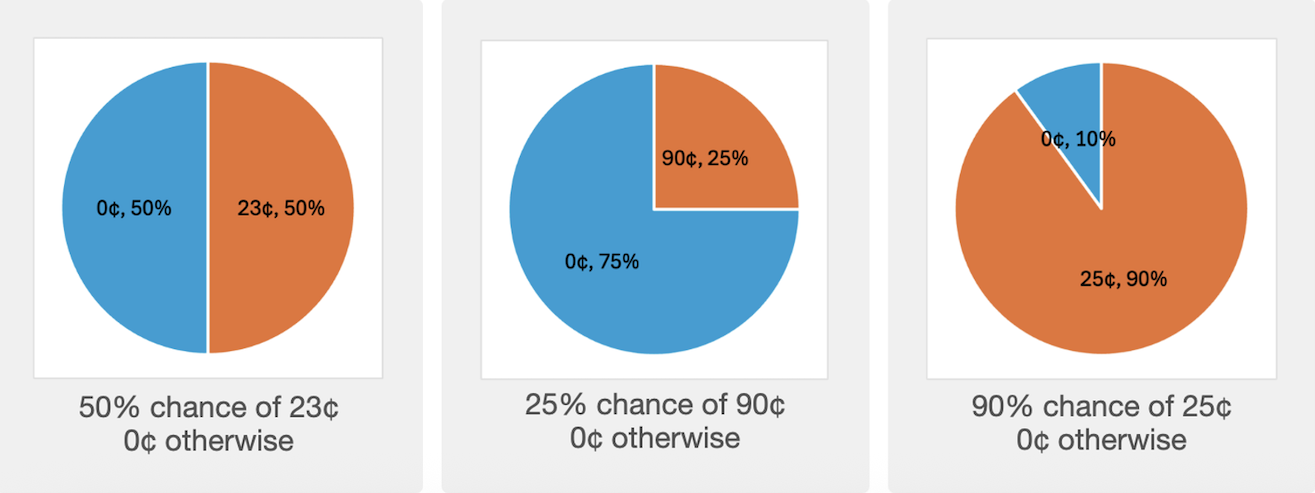
\includegraphics[width=1\textwidth]{Control.png}
\end{center}
\end{frame}

\begin{frame}{Study 1: Treatment Trails: targets Safe lottery}
\phantomsection\label{study-1-treatment-trails-targets-safe-lottery}
\begin{center}
  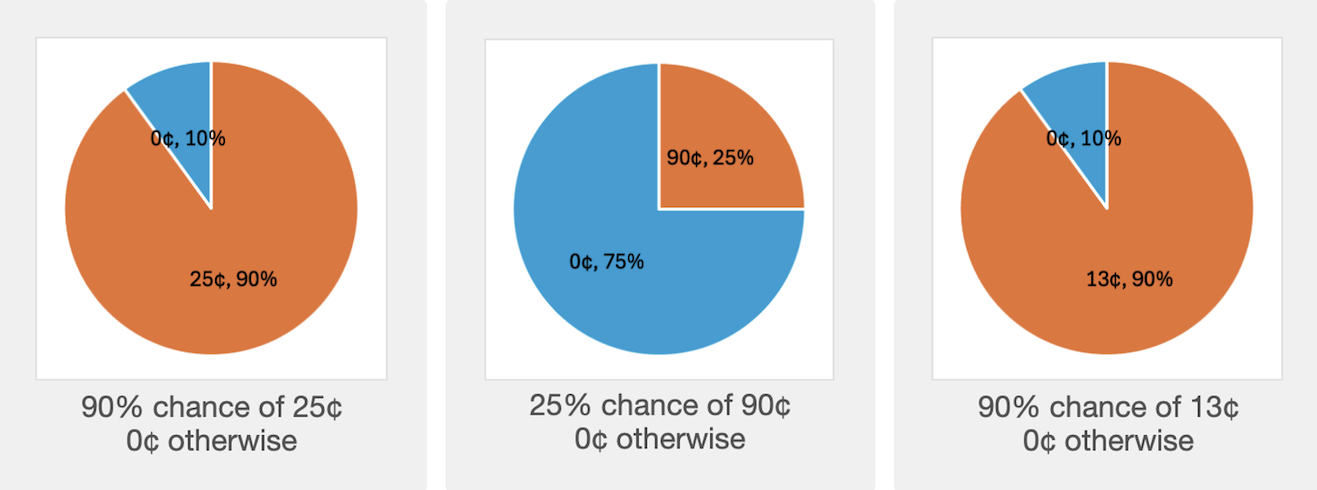
\includegraphics[width=1\textwidth]{Treatment_Risk_Averse.png}
\end{center}
\end{frame}

\begin{frame}{Study 1: Treatment Trails: targets Risky lottery}
\phantomsection\label{study-1-treatment-trails-targets-risky-lottery}
\begin{center}
  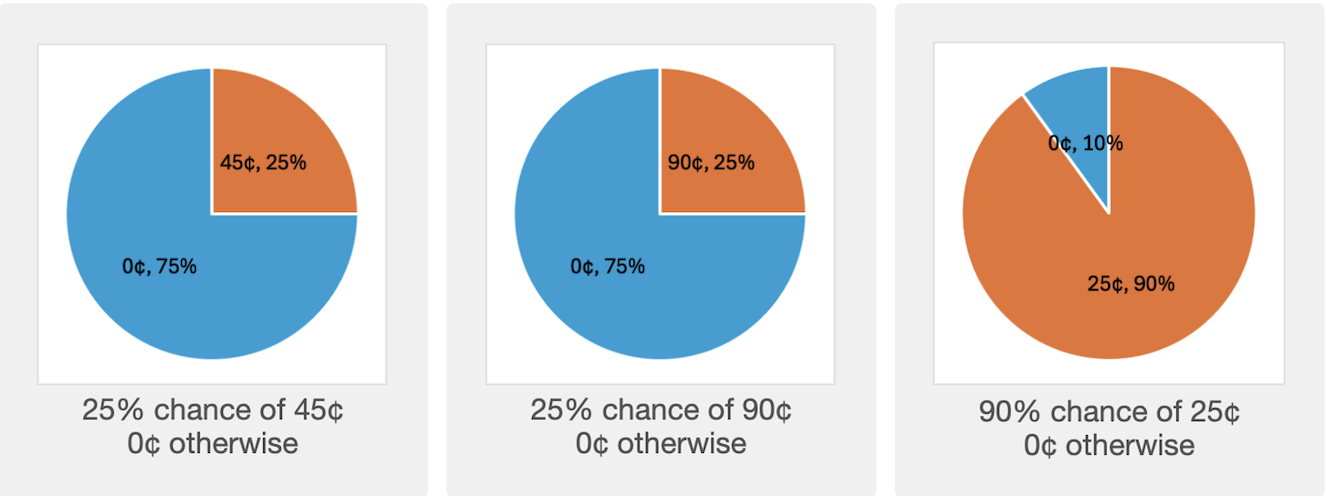
\includegraphics[width=1\textwidth]{Treatment_Risk_Seeking.png}
\end{center}
\end{frame}

\begin{frame}{Study 1: Design}
\phantomsection\label{study-1-design}
\begin{itemize}
  \item 600 participants from Prolific
  \pause
  \item Within subject treatment
  \begin{itemize}
    \pause
    \item 10 trails of lottery decision
    \item 5 unique pairs of Focal and Non-focal lotteries
    \item Along with either a Treatment or a Control Decoy
  \end{itemize}
  \pause
  \item Between subject condition
  \begin{itemize}
    \pause
    \item \textbf{Risky} Treatment Decoy targets the risky lottery
    \item \textbf{Safe} Treatment Decoy targets the safe lottery
  \end{itemize}
  \pause
  \item Exclude participants who choose the decoy more than 5 times
\end{itemize}

\vfill

\hfill \tiny *All studies preregistered on AsPredicted
\end{frame}

\begin{frame}{Different levels of tradeoffs}
\phantomsection\label{different-levels-of-tradeoffs}
\begin{itemize}
  \item 95\% of 20¢; 20\% of 95¢
  \item 90\% of 25¢; 25\% of 90¢
  \item 85\% of 30¢; 30\% of 85¢
  \item 80\% of 35¢; 35\% of 80¢
  \item 75\% of 40¢; 40\% of 75¢
\end{itemize}
\end{frame}

\begin{frame}{Study 1: Hypothesis}
\phantomsection\label{study-1-hypothesis}
\begin{itemize}
  \item Can the Treatment Decoy increase the likelihood of choosing the Focal lottery?
  \pause
  \item Does the effect depend on specific characteristic in lottery pairs?
  \pause
  \item Whether Treatment Decoy is better at enhancing risky lotteries or safe lotteries?
\end{itemize}
\end{frame}

\section{Results}\label{results}

\begin{frame}{Study 1: Seperated by Conditions}
\phantomsection\label{study-1-seperated-by-conditions}
\begin{flushright}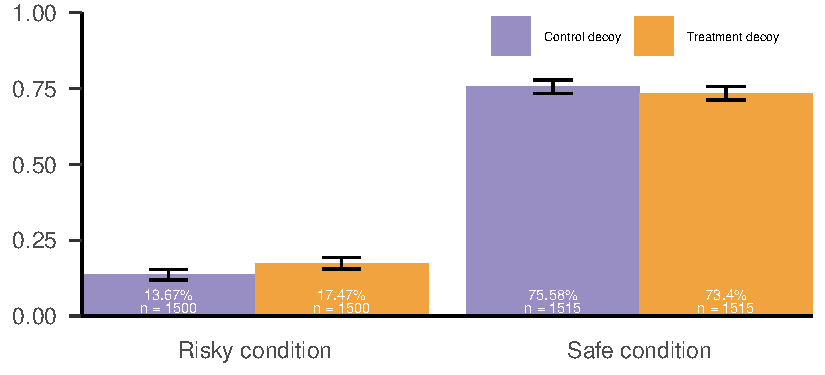
\includegraphics{BE_Lab_1023_files/figure-beamer/unnamed-chunk-1-1} \end{flushright}
\end{frame}

\begin{frame}{Study 1: No and Opposite Preference Reversal (Treatment)}
\phantomsection\label{study-1-no-and-opposite-preference-reversal-treatment}
\begin{flushright}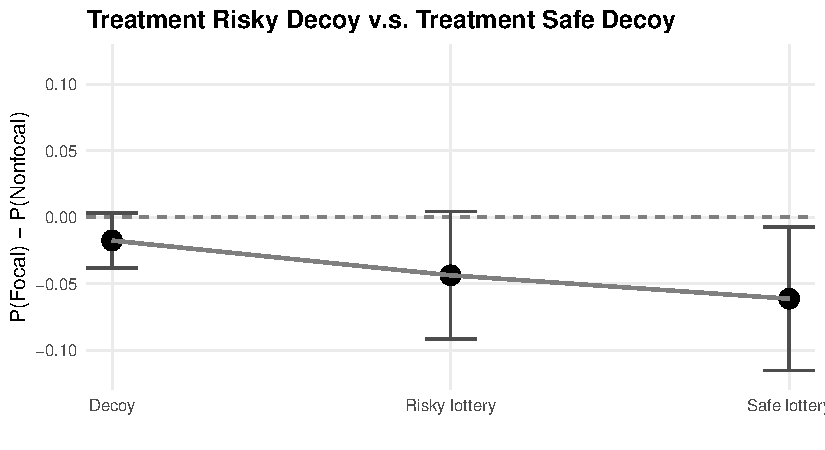
\includegraphics{BE_Lab_1023_files/figure-beamer/unnamed-chunk-3-1} \end{flushright}
\end{frame}

\begin{frame}{No Heterogenous Effect Across Pairs}
\phantomsection\label{no-heterogenous-effect-across-pairs}
\begin{flushright}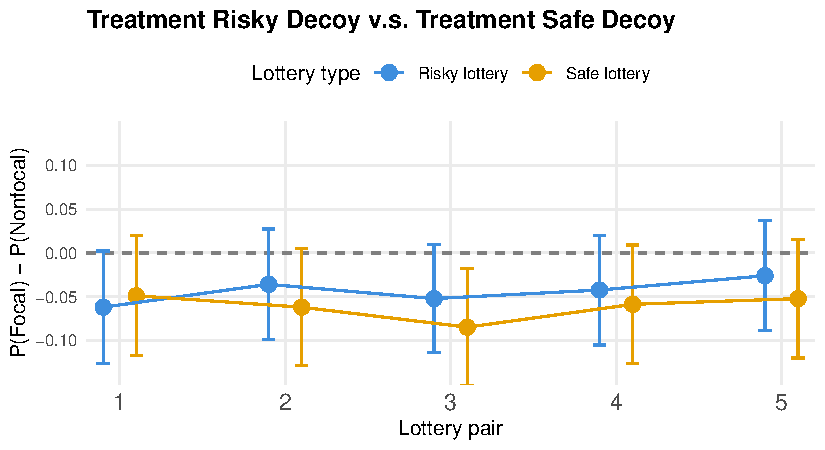
\includegraphics{BE_Lab_1023_files/figure-beamer/unnamed-chunk-5-1} \end{flushright}
\end{frame}

\begin{frame}{Study 1: Risky Decoy: Treatment v.s. Control}
\phantomsection\label{study-1-risky-decoy-treatment-v.s.-control}
\begin{flushright}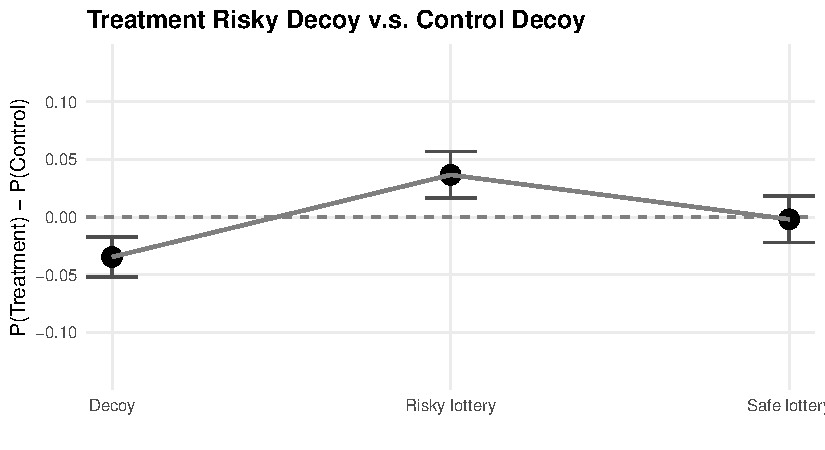
\includegraphics{BE_Lab_1023_files/figure-beamer/unnamed-chunk-7-1} \end{flushright}
\end{frame}

\begin{frame}{Study 1: Safe Decoy: Treatment vs.~Control}
\phantomsection\label{study-1-safe-decoy-treatment-vs.-control}
\begin{flushright}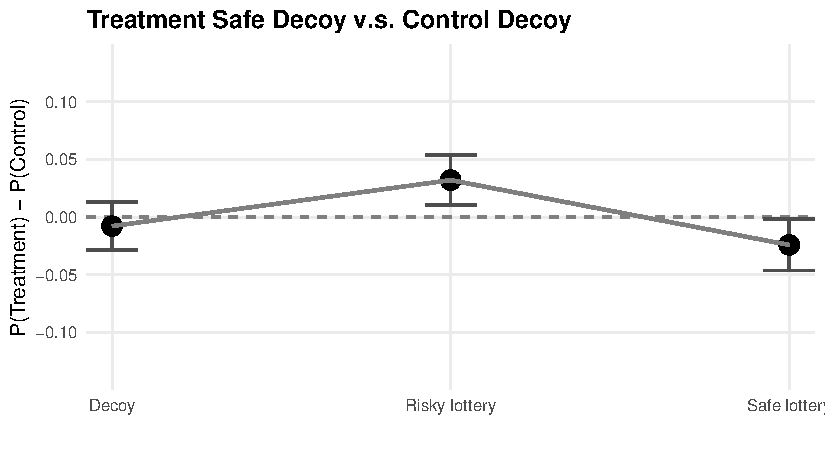
\includegraphics{BE_Lab_1023_files/figure-beamer/unnamed-chunk-9-1} \end{flushright}
\end{frame}

\begin{frame}{Study 1: Conclusion}
\phantomsection\label{study-1-conclusion}
\begin{flushleft}
  \textbf{No significant preference reversal}
  \begin{itemize}
    \item Compared with risky decoy, Safe decoy slightly \textit{reduced} safe choice
    \item AE not robust to visual representation (Frederick et al., 2014)
  \end{itemize}
\end{flushleft}

\pause
\begin{flushleft}
  \textbf{No heterogenous effect across pairs characteristics}
  \begin{itemize}
    \item Distance between competing options didn't matter
    \item No support for similar effect on perceptual task (Farmer et al., 2016)
    \item Similarity doesn't make the preference easier shift
  \end{itemize}
\end{flushleft}

\pause
\begin{flushleft}
  \textbf{Control decoy is "inadvertently" dominated by safe lottery on both attributes}
  \begin{itemize}
    \item Control decoy \textit{boosted} safe choices more than safe decoy
    \item Must decoys be strictly dominated in \textit{both} attributes?
    \item Couldn't similarity itself trigger comparison?
  \end{itemize}
\end{flushleft}
\end{frame}

\begin{frame}{Study 1: Make One Attractive or Avoid Worst Option?}
\phantomsection\label{study-1-make-one-attractive-or-avoid-worst-option}
\begin{flushleft}
  \textbf{47\% \$23 v.s. 19\% \$57}
  \begin{itemize}
    \item Hard to tell which has higher EV
    \item Decoy 19\% \$28 may work
    \item At least I won't choose the worst option
  \end{itemize}
\end{flushleft}

\pause
\begin{flushleft}
  \textbf{47\% \$23 v.s. 23\% \$47}
  \begin{itemize}
    \item They obviously have the same EV
    \item Decoy 23\% \$23 may not work
    \item When competing options are objectively equivalent
  \end{itemize}
\end{flushleft}

\pause
\begin{flushleft}
  \textbf{Moving away from single choice DV}
  \begin{itemize}
    \item Elicit WTP?
    \item Ask for rankings?
    \item Allow multiple choices?
  \end{itemize}
\end{flushleft}
\end{frame}

\begin{frame}{Moving Forwards}
\phantomsection\label{moving-forwards}
\pause
\begin{flushleft}
  \textbf{What do you make of the results?}
\end{flushleft}
\begin{itemize}
  \item Risky decoy lowered "mistake" rate
  \item While safe decoy backfired
\end{itemize}

\pause
\begin{flushleft}
  \textbf{How to position this study?}
\end{flushleft}
\begin{itemize}
  \item Reference-dependent risk preference
  \item Regret theory — state-wise comparison
  \item Heuristics and biases — reduced mistakes
\end{itemize}

\pause
\begin{flushleft}
  \textbf{Next step?}
\end{flushleft}
\begin{itemize}
  \item Refine experimental design — a better control?
  \item More experimental or theoretical?
  \item Test in more realistic settings?
\end{itemize}
\end{frame}

\section{Appendix}\label{appendix}

\begin{frame}{Study 1: Frequency table}
\phantomsection\label{study-1-frequency-table}
\begin{table}
\centering
\begin{tabular}{lllll}
\toprule
Treatment & Condition & Decoy & Risky & Safe\\
\midrule
Control & Safe & 6.1\% & 18.6\% & 75.2\%\\
Treatment & Safe & 5.4\% & 21.8\% & 72.8\%\\
Control & Risky & 7.1\% & 13.8\% & 79.2\%\\
Treatment & Risky & 3.6\% & 17.5\% & 79\%\\
\bottomrule
\end{tabular}
\end{table}

\vfill

\hfill \tiny *Full sample without excluding any participant
\end{frame}

\begin{frame}{Appendix: Switch to Focal, Conditioned on Not Choosing
Focal in Control}
\phantomsection\label{appendix-switch-to-focal-conditioned-on-not-choosing-focal-in-control}
\begin{flushright}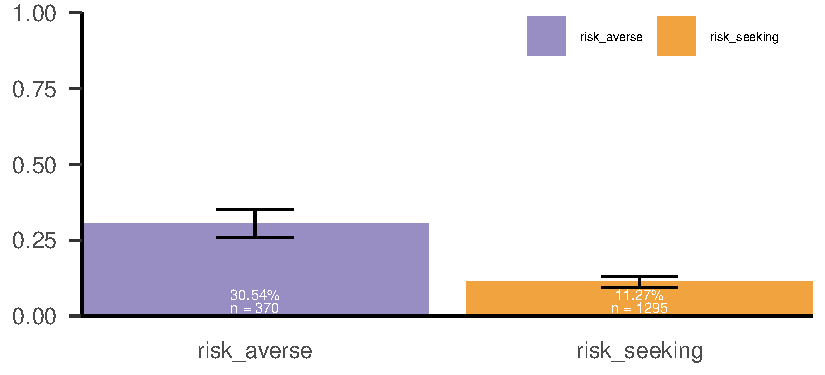
\includegraphics{BE_Lab_1023_files/figure-beamer/unnamed-chunk-11-1} \end{flushright}
\end{frame}

\begin{frame}{Appendix: Move away from Focal, Conditioned on Already
Choosing Focal in Control}
\phantomsection\label{appendix-move-away-from-focal-conditioned-on-already-choosing-focal-in-control}
\begin{flushright}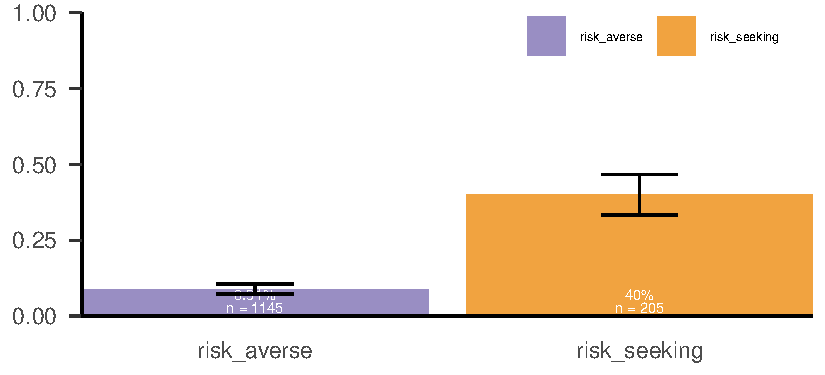
\includegraphics{BE_Lab_1023_files/figure-beamer/unnamed-chunk-12-1} \end{flushright}
\end{frame}

\begin{frame}{Appendix: Heat Map -- Safe Condition}
\phantomsection\label{appendix-heat-map-safe-condition}
\begin{table}
\centering
\caption{\label{tab:unnamed-chunk-13}Safe condition}
\centering
\begin{tabular}[t]{llll}
\toprule
Control & Decoy & Risky & Safe\\
\midrule
Decoy & 10.5\% & 59.3\% & 30.2\%\\
Risky & 6.7\% & 62.7\% & 30.6\%\\
Safe & 3.8\% & 8.9\% & 87.2\%\\
\bottomrule
\end{tabular}
\end{table}
\end{frame}

\begin{frame}{Appendix: Heat Map -- Risky Condition}
\phantomsection\label{appendix-heat-map-risky-condition}
\begin{table}
\centering
\caption{\label{tab:unnamed-chunk-14}Risky condition}
\centering
\begin{tabular}[t]{llll}
\toprule
Control & Decoy & Risky & Safe\\
\midrule
Decoy & 10.2\% & 38.6\% & 51.1\%\\
Risky & 3.4\% & 56.6\% & 40\%\\
Safe & 1.7\% & 9.3\% & 89\%\\
\bottomrule
\end{tabular}
\end{table}
\end{frame}

\end{document}
